Electrostatic Actuators (EA) are an interesting alternative for the control of the test masses, respect to the widely used coil-magnet pairs.

Such solution was already applied for the GEO 600 detector \cite{GeoCal} and it is under study also for other detectors, currently adopting coil-magnet pair actuators. The use of EA offers several advantages. The first one is the possibility to keep the mirrors under control without the need of gluing the magnets on the mirror bulk, saving, in this way, the mechanical quality of the test masses and, as a consequence, reducing the final thermal noise \cite{Amico}. Another advantage is the strong reduction of the coupling with external magnetic fields, that is an important issue for magnetic actuators, since no direct coupling is anymore possible in the case of EA. Another possible advantage, mainly for third generation detectors, is linked to the possibility to control the suspended test mass, in science mode, only from the previous suspension stage, avoiding the need of a reference mass. In this case an electrostatic actuator, fixed on ground, represents the simplest way for the lock acquisition without adding any extra noise when the control is transferred to the upper stage.

The working principle of an electrostatic actuator is simply described by standard electrostatic, giving, for a device of capacitance $C$, polarized at fixed voltage $V$, a resulting force along the $x$ axis equal to:
\begin{equation}
\label{eqn:force_base}
F_x = - \frac{1}{2} \left| \frac{\mathrm{d} C}{\mathrm{d} x} \right| V^2=-\alpha V^2
\end{equation}
where the capacitance is supposed to vary by changing the system characteristics along the $x$ axis while the minus sign is due to the characteristic of such forces, that are always attractive.
In the case of actuator for suspended dielectric mirrors, such devices mainly consist in a set of close conductive strips, arranged in a suitable geometry, alternately polarized at two different voltages.
The strips, together with the dielectric suspended test mass, placed at distance a $x$ with respect to the actuator plane, constitute a capacitor, with a capacitance variable by changing the distance of the test mass with respect to the actuator.

The deduction of the theoretical expression of the capacitance, for such system, is described in \cite{Grasso}. It can be written as:
For the simplest geometry, i.e.\ a set of $N$ parallel conductive strips with period $b$, rectangular in shape, of length $L$ and width $a$, laying on a substrate with relative dielectric constant $\epsilon_{s}$, placed at distance $x$ from the test mass having a relative dielectric constant $\epsilon_{m}$, the capacitance can be written as:
\begin{equation}
\label{eqn:c_exp}
C(x)=C_\infty \alpha_m\left(\tilde{a},\tilde{x},\epsilon_m\right)
\end{equation}
where $\tilde{a}=a/b$ is the normalized strip width, $\tilde{x}=x/b$ is the normalized distance, {$\alpha_m$ is a function of the listed parameters describing the effect of the mirror at distance $x$, and $C_\infty$ is the capacitance of the isolated actuator (i.e.\ with $x\rightarrow+\infty$).
This expression is calculated in the approximation of infinitely long strips and taking into account only the contribution of the first image charges, both for the substrate and for the mirror. As a consequence the capacitance of real devices become different from the this value for small values of $x$ with respect to $b$ due to the increasing weight of border effects and image charges as the distance decreases \cite{Grasso}. 

The force expression (\ref{eqn:force_base}) has to be modified to consider also the presence of a stray electric charge $q$ on the dielectric mass. In this case, by making the simple approximation that the electric field is proportional to the polarization voltage applied to the actuator, it is possible to write:
\begin{equation}
\label{eqn:total_force}
F_x = -\alpha V^2 +\beta V
\end{equation}
where the factor $\beta$ is, in general, a function of the charge $q$, the distance $x$ and the geometry of the actuator.
The effects of this term were already observed on a similar set-up \cite{Mortonson}, and some techniques for its mitigation were already developed \cite{GeoCharge}. To reduce the effect of the stray charges, it is also possible to modulate the driving signal, to obtain a zero averaged contribution of the linear term of the  actuation force even in presence of charges on the test masses \cite{ElDrive}. This driving technique was already successfully experimented in the control of a bench top Michelson interferometer with a suspended mirror controlled by a such EA \cite{ElAct}.

To clarify this approach, let $A(t)$ be the driving signal we want to apply on the test mass, $A_{DC}$ the voltage bias and $f_M=\omega_M/2\pi$ the modulation frequency of the full driving signal. The square root is computed and sent, with the modulation, to the actuator driver. In this way the voltage applied to the actuator is:
\begin{equation}
\label{eqn:voltage}
V=G\sqrt{A_{DC}+A(t)}\cos{\omega_M t}
\end{equation}
where $G$ is the gain of the EA driver. With this voltage, the force exerted on the test mass becomes:
\begin{equation}
\label{eqn:elac_force}
F=-\frac{1}{2}\alpha G^2\left( A_{DC}+A(t)\right)\left(1+\cos{2\omega_M t}\right)+\beta G \sqrt{A_{DC}+A(t)}\cos{\omega_M t}
\end{equation}
If the modulation frequency is chosen at enough high frequency to have negligible effects on the test mass motion and the frequency content of the driving signal is much smaller with respect to $f_M$, the main contribution of the force (\ref{eqn:elac_force}) only consists of a DC bias term plus a term proportional to the driving signal $A(t)$. This is the required behavior for such actuator.

The characterization of an EA with such driving technique is described in \cite{ElDrive}.
\begin{figure}
\begin{minipage}{0.47\textwidth}
\begin{center}
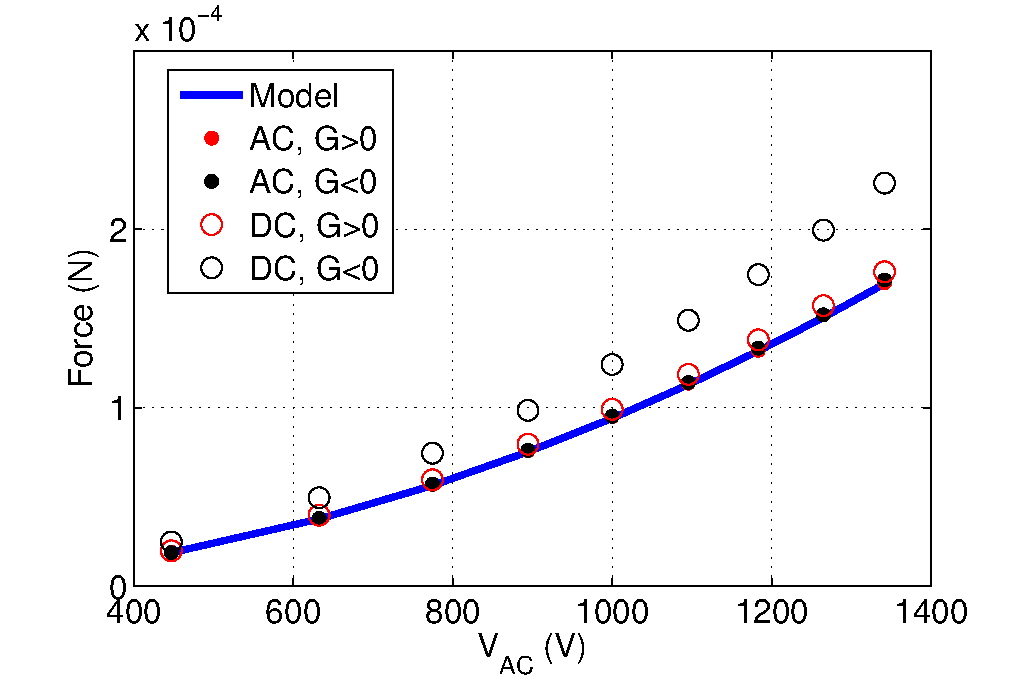
\includegraphics[width=\textwidth]{Measure1.pdf}   
\caption{ \label{fig:measure1} Comparison between the model and the force measured, in different bias conditions, for a excitation with $f=0.1$ Hz.}
\end{center}
\end{minipage}
\hspace{0.5cm}
\begin{minipage}{0.47\textwidth}
\begin{center}
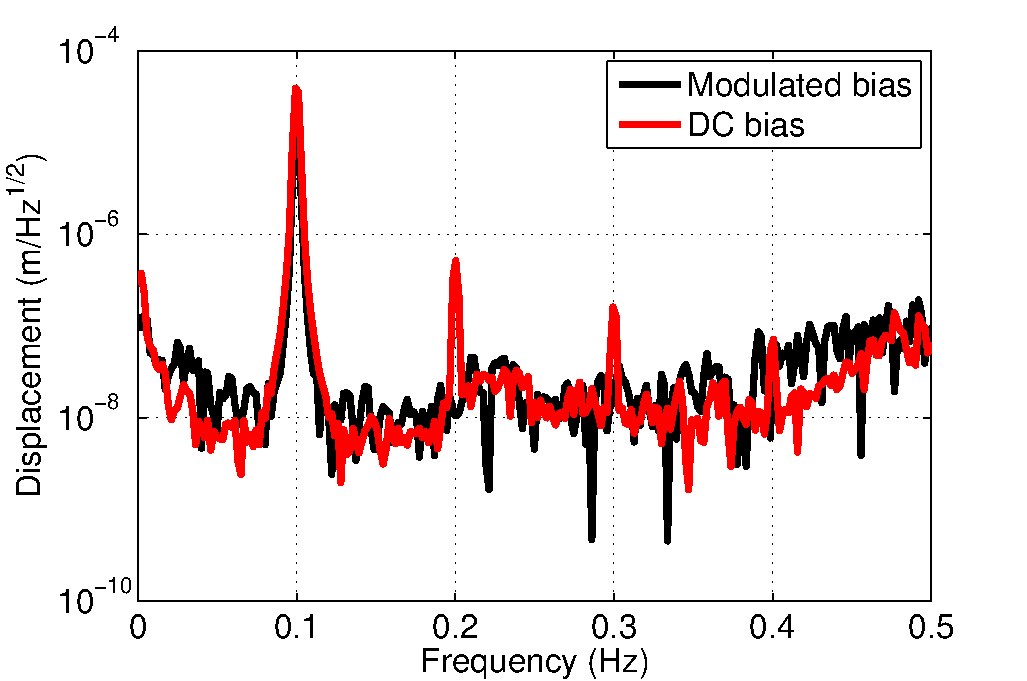
\includegraphics[width=\textwidth]{Charge.pdf}
\caption{ \label{fig:charge} Spectra of the test mass displacement with the same actuation force, at $f=0.1$ Hz in two different bias conditions.}
\end{center}
\end{minipage}
\end{figure}
The most interesting results are related to some observed deviation from the theoretical model. The measurements are shown in figure \ref{fig:measure1}. The filled dots represent the force measured in AC bias, both with positive or negative $G$, while the open circles are the force measured in DC bias with different sign of $G$. The deviation from the foreseen behavior, clearly visible for all the points in DC bias, in particular in the case of negative $G$, is due to the presence of spurious charges on the dielectric suspended mass. In fact in this case, equation (\ref{eqn:elac_force}) becomes:
\begin{equation}
\label{eqn:dc_force}
F=-\alpha G^2\left( A_{DC}+A_{AC}\cos{\omega t}\right)+\beta G \sqrt{A_{DC}+A_{AC}\cos{\omega t}}
\end{equation}
and a not negligible contribution could arise from the last term. Moreover this contribution depends on $G$ as confirmed by the results. The two opposite polarizations, for the AC bias, give instead the same results, as the experimental measurements are practically overlapped. This confirms the effectiveness of the alternate bias technique that is insensitive to any static stray charge present on the test mass.

Following the (\ref{eqn:dc_force}) a larger disagreement would be expected also for the case of DC bias with positive $G$, but  one should consider that the description of the electrical field between the EA and the test mass is very roughly approximated in the model; moreover a slight dependence of $\beta$ from the sing of $G$ is expected. More investigations are need in this direction which also require some upgrade in the experimental set-up, as the possibility to change the distance between the EA and the test mass without opening the chamber and changing, in this way, the amount of charges on the mass.
The displacement spectra, in case of measurements in DC bias conditions, also show additional lines placed at multiple frequency respect to the one injected by the signal. These lines disappear if the measurement is performed in AC bias as shown in figure \ref{fig:charge}.

Starting from theoretical model, and on the basis of the previous results, it not too difficult to effectively design the electrostatic actuation system for ET. By assuming a mirror mass of 200 Kg (it is slightly higher for LF-ET, but the difference is not very relevant), a wire length of the last stage of 2 m and a conservative residual motion of the test mass  $x \sim10 \mu$m, the minimum force required for damping the mirror motion is:
\begin{equation}
F \sim m\omega_0^2 x = 250 \mu\textrm{N}
\end{equation}
Since the beam radius is about 9 cm and the mirror diameter is 45 cm (in the worst case) the maximum reasonable residual space useful for the EA is about 10 cm. Moreover the distance between the test mass and the actuator has to be at least 5 mm, in order to reduce the damping from the residual pressure, and this also fix the period of the electrodes strip, that has to be close to the mirror-actuator distance to enhance the field fringes.
From these figures it results that each actuator can be composed by 5 strips large 4 mm arranged in concentric arches. For such pattern the model provide $\alpha=1.8\cdot10^{-10}$ N/V$^2$. By using the equation (\ref{eqn:force_base}) it results that the required force, using 4 pattern, can be achieved with a maximum voltage of about 600 V, that is a good value for voltage amplifiers with low electronic noise and large bandwidth.
After the lock acquisition the actuation noise can be easily reduced by reducing the voltage bias of the actuator until few volts, hence by reducing the noise of two order of magnitude. Of course, in case of full locking reallocation at the marionetta level the electrostatic actuator can even be switched off and no actuation noise is introduced.